%%%%%%%%%%%%%%%%%%%%%%%%%%%%%%%%%%%%%%%%%%%%%%%%%%%%%%%%%%%%%%
%%%%		PLANTILLA LATEX PARA INFORMES
%%%%			LATEX REPORT TEMPLATE
%%%%
%%%%	Autor	: Carlos Gonzalez Cortes
%%%%	Correo	: carlgonz@ug.uchile.cl
%%%%	Version	: 1.0
%%%%
%%%%	Notas	: Este codigo se entrega tal cual es y sin
%%%%			  ningun tipo de garantia. Sientase libre de
%%%%			  modificar y compartir.(acentos omitidos en
%%%%			  los comentarios por compatibilidad)
%%%%
%%%%%%%%%%%%%%%%%%%%%%%%%%%%%%%%%%%%%%%%%%%%%%%%%%%%%%%%%%%%%%




\documentclass[11pt,letterpaper]{article}
\usepackage[spanish]{babel}
%\usepackage[ansinew]{inputenc}
\usepackage[utf8]{inputenc}
% \usepackage[latin1]{inputenc}
\usepackage[letterpaper,includeheadfoot, top=0.5cm, bottom=3.0cm, right=2.0cm, left=2.0cm]{geometry}
\renewcommand{\familydefault}{\sfdefault}

\usepackage{graphicx}
\usepackage{color}
\definecolor{deepblue}{rgb}{0,0,0.5}
\definecolor{deepred}{rgb}{0.6,0,0}
\definecolor{deepgreen}{rgb}{0,0.5,0}
\usepackage{hyperref}
\usepackage{amssymb}
\usepackage{url}
%\usepackage{pdfpages}
\usepackage{fancyhdr}
\usepackage{hyperref}
\usepackage{subfig}
\DeclareFixedFont{\ttb}{T1}{txtt}{bx}{n}{9} % for bold
\DeclareFixedFont{\ttm}{T1}{txtt}{m}{n}{9}  % for normal
\definecolor{mauve}{rgb}{0.58,0,0.82}

\usepackage{listings} %Codigo
\lstset{
language=scala,
basicstyle=\ttm,
otherkeywords={this, case},             % Add keywords here
keywordstyle=\ttb\color{deepblue},
%emph={MyClass,__init__},          % Custom highlighting
%emphstyle=\ttb\color{deepred},% Custom highlighting style
stringstyle=\color{mauve},
commentstyle=\color{deepgreen},
frame=tb,                         % Any extra options here
showstringspaces=false            %
}

\begin{document}
%\begin{sf}
% --------------- ---------PORTADA --------------------------------------------
\newpage
\pagestyle{fancy}
\fancyhf{}
%-------------------- CABECERA ---------------------
\fancyhead[L]{ 
\includegraphics[scale=0.9]{img/logo.pdf} }
%------------------ TÍTULO -----------------------
\vspace*{6cm}
\begin{center}
\Huge  {Tarea 4}\\
\vspace{1cm}
\huge {Programación genética y AST}\\
%\vspace{1cm}
%\small {Título pe} \\
\end{center}
%----------------- NOMBRES ------------------------
\vfill
\begin{flushright}
\begin{tabular}{ll}
Autor: & Matías Meneses C.\\
Profesor: & Alex Bergel\\
& \today\\
& Santiago, Chile.
\end{tabular}
\end{flushright}

% ·············· ENCABEZADO - PIE DE PAGINA ············
\newpage
\pagestyle{fancy}
\fancyhf{}

%Encabezado
%\fancyhead[L]{\rightmark}
\fancyhead[L]{\small \rm \textit{Sección \rightmark}} %Izquierda
\fancyhead[R]{\small \rm \textbf{\thepage}} %Derecha


\fancyfoot[L]{\small \rm \textit{Redes Neuronales y Programación Genética}} %Izquierda
\fancyfoot[R]{\small \rm \textit{Tarea 4 - Programación Genética y AST}} %Derecha
%\fancyfoot[C]{\thepage} %Centro

\renewcommand{\sectionmark}[1]{\markright{\thesection.\ #1}}
\renewcommand{\headrulewidth}{0.5pt}
\renewcommand{\footrulewidth}{0.5pt}

% =============== INDICE ===============

\tableofcontents
%\listoffigures

% =============== SECCION ===============
\newpage
\section{Introducción}
El objetivo de esta tarea es implementar un algoritmo de programación genética para 
árboles de operaciones binarias, con el objetivo de estudiar la implementación práctica de 
programación genética.
\subsection{Software utilizado}
Se utilizó el lenguaje de programación Scala para la implementación del AST y los test unitarios. Se 
eligió este lenguaje debido a la facilidad para realizar Pattern Matching sobre clases, y para variar 
de las tareas anteriores en donde se utilizó Python. Se utilizó SBT como gestor de paquetes y compilación.

\section{Estructura de Árbol}

Scala permite el uso de \textit{case classes} para poder realizar pattern matching de forma 
intuitiva y funcional.

\begin{lstlisting}
trait ArithmeticNode {

    def evaluate(): Int = this match {
      case Number(n) => n
      case Plus(n1, n2) => n1.evaluate() + n2.evaluate()
      case Minus(n1, n2) => n1.evaluate() - n2.evaluate()
      case Mult(n1, n2) => n1.evaluate() * n2.evaluate()
      // se establece que x / 0 es x
      case Div(n1, n2) =>
        if (n2.evaluate() == 0) n1.evaluate()
        else n1.evaluate() / n2.evaluate()
    }

    ...
}

case class Number(n: Int) extends ArithmeticNode
case class Plus(l: ArithmeticNode, r: ArithmeticNode) extends ArithmeticNode
case class Minus(l: ArithmeticNode, r: ArithmeticNode) extends ArithmeticNode
case class Mult(l: ArithmeticNode, r: ArithmeticNode) extends ArithmeticNode
case class Div(l: ArithmeticNode, r: ArithmeticNode) extends ArithmeticNode
\end{lstlisting}

Se definió además un trait (interfaz) AlgebraicNode, cuyas terminales son identificadores en lugar de 
números.\\

Se implementaron métodos para generar árboles aleatorios, y reemplazar de forma aleatoria un subárbol de 
un árbol por otro árbol, lo cual es útil para la implementación de los algoritmos genéticos. Además, se implementaron métodos para obtener la altura del árbol y para imprimirlo en pantalla de forma legible.

\section{Algoritmos Genéticos}

\subsection{Selection}
La función de selección recibe como parámetro una lista de árboles, la cantidad de árboles a seleccionar y una función de fitness $\text{Node}\rightarrow \mathbb{Z}$, y retorna una lista con los árboles seleccionados, ordenados por mejor fitness.

\subsection{Crossover}
La función de crossover recibe como parámetro una lista de árboles (padres) y el número de hijos a 
generar, y retorna una lista con los hijos generados. La función toma dos padres al azar de la lista de padres, y luego reemplaza un subárbol aleatorio del segundo padre en el primer padre, 
para formar a un hijo, el cual tiene una probabilidad de 1\% de ser mutado. 
Se repite este proceso hasta generar todos los hijos.

\subsection{Mutation}
La función de mutación recibe como parámetro un árbol y retorna un árbol mutado. El árbol mutado es 
el resultado del reemplazo de un subárbol aleatorio del árbol por un árbol generado aleatoriamente.

\section{Experimentos}
En esta oportunidad, los experimentos se implementaron como test unitarios.


\subsection{Primer Experimento}
En el primer experimento se utiliza el árbol aritmético (las terminales son números hasta 100). La idea es que 
a partir de 20 árboles aleatorios, evolucionen para formar un árbol que evalúe a un número entre $40$ y $50$.\\

La función de fitness para este problema es la distancia al punto medio del intervalo. A menor fitness, 
más cerca de la respuesta.
\begin{lstlisting}
val fitness = (n: ArithmeticNode) => Math.abs(n.evaluate() - 45.0)
\end{lstlisting}

Se itera siguiendo los pasos del algoritmo genético, hasta entontrar un árbol que solucione el problema. Se varió la profundidad de los árboles generados aleatoriamente para analizar su impacto.

\subsection{Segundo Experimento}
En el segundo experimento se utiliza el árbol algebraico (las terminales son variables $x, y, z$). La 
idea es que a partir de 20 árboles aleatorios, evolucionen para formar un árbol que, dado 
$x = 1, y = 2, z = 3$, evalúe a un número entre $40 y 50$.\\

La función de fitness es similar al experimento anterior.
\begin{lstlisting}
val fitness = (n: AlgebraicNode) => Math.abs(n.evaluate(1,2,3) - 45.0)
\end{lstlisting}

Se itera siguiendo los pasos de algoritmo genético, hasta encontrar un árbol que solucione el problema.

\section{Resultados}

\begin{figure}[ht!]
\centering 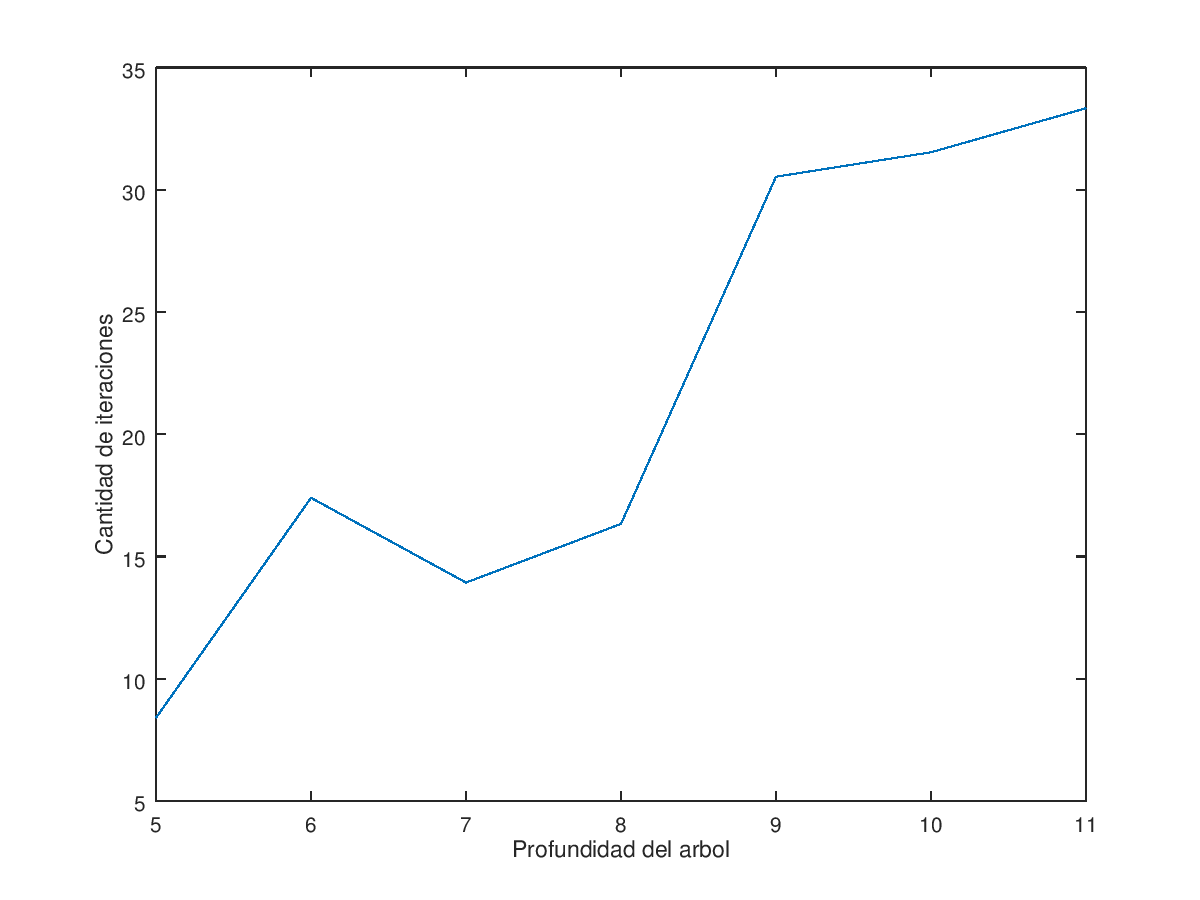
\includegraphics[width=\textwidth]{img/depth.png}
\caption{Cantidad de iteraciones hasta encontrar la solución por altura del árbol} \label{img1}
\end{figure}

\clearpage

\begin{figure}[ht!]
\centering 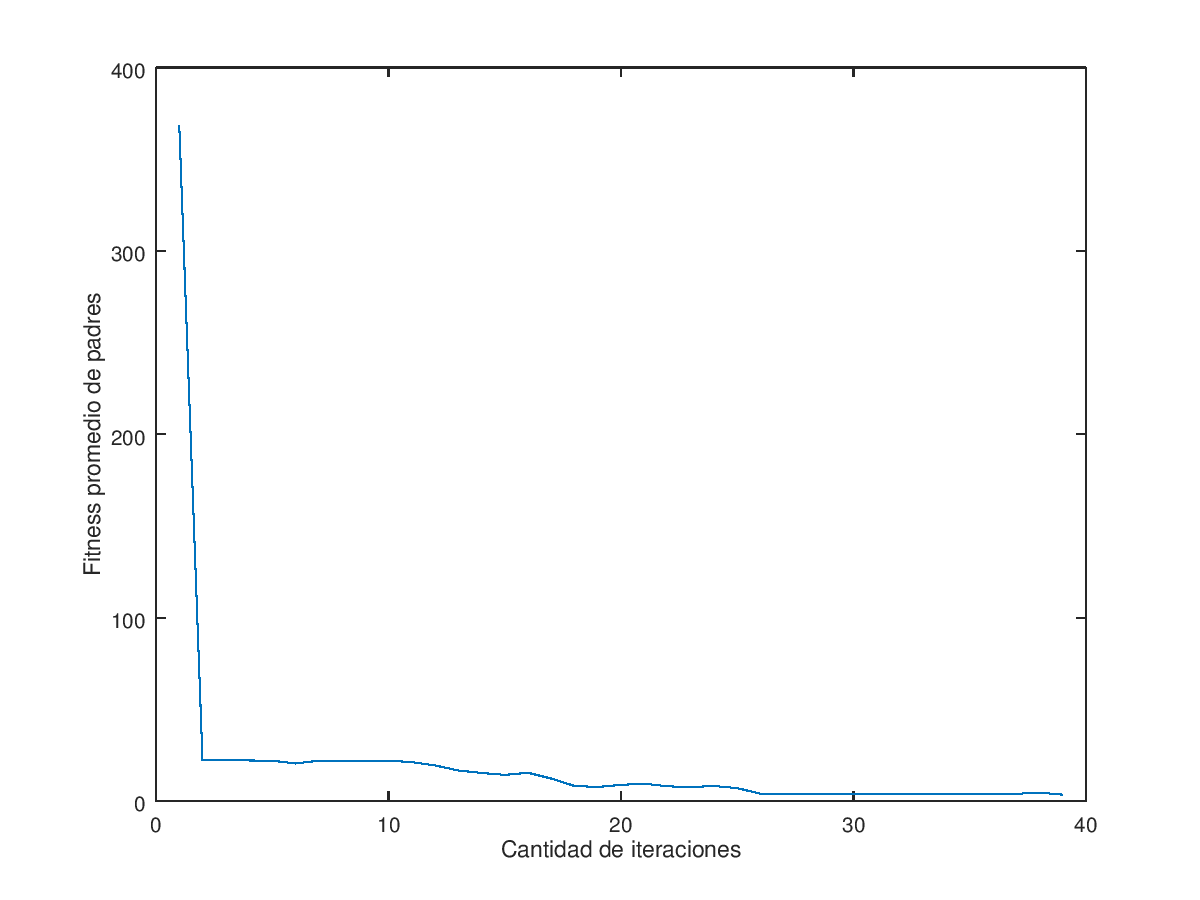
\includegraphics[width=\textwidth]{img/fitness.png}
\caption{Fitness promedio de padres por cantidad de iteraciones} \label{img2}
\end{figure}

\clearpage
\begin{figure}[ht!]
\centering 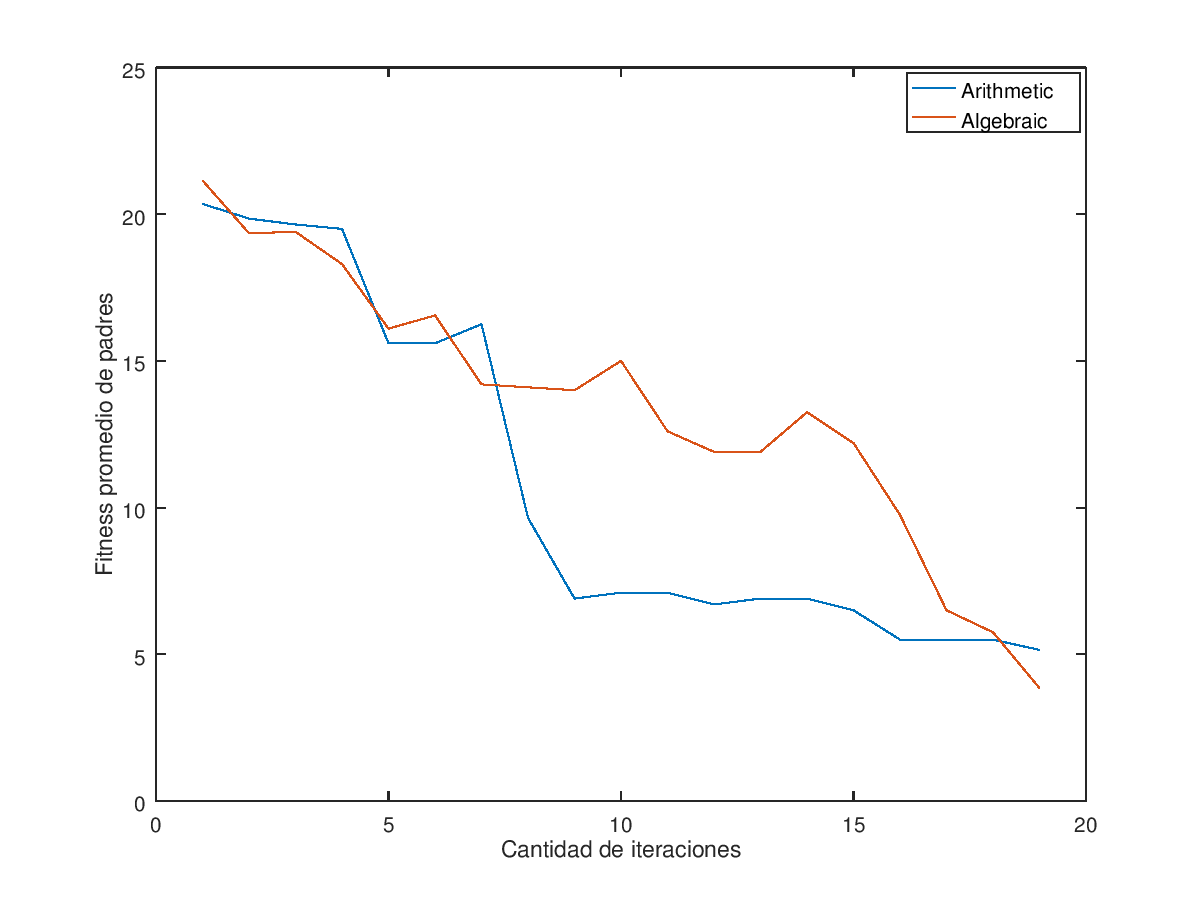
\includegraphics[width=\textwidth]{img/comp.png}
\caption{Fitness promedio de padres por cantidad de iteraciones (sin singularidad)} \label{img3}
\end{figure}
\clearpage

\section{Análisis de Resultados}
Se puede ver de la figura 1, que mientras mayor es la altura de los árboles generados, mayor es la 
cantidad de iteraciones requerida para encontrar una solución, lo cual era de esperar, puesto que 
mientras más complejos son los programas, mayor es la cantidad de outputs que puede generar, por lo que será más difícil acotar la solución.\\

Se puede ver de las figuras 2 y 3 que el algoritmo genético logra aproximar las soluciones en cada 
iteración. En todas las ejecuciones, el fitness promedio de la primera iteración siempre era un valor 
muy alejado de la solución, por lo que se removió en la figura 3 para visualizar de mejor forma la 
variación. Esta figura también compara las iteraciones para los dos tipos de árboles implementados, 
no habiendo diferencias significativas.

\section{Conclusión}
Se concluye que el algoritmo genético fue capaz de generar programas que solucionan las ecuaciones 
objetivo, en ambos ejemplos que utilizan terminales distintas. Se espera que, ante un AST con mayor 
cantidad de tipos de nodos, también se puedan generar programas que aproximen a una solución.\\

Se cumplió el objetivo propuesto para esta tarea.

% ============= FIN DE DOCUMENTO ==============
\end{document}

% % ················ IMAGEN ·················
% \begin{figure}[ht!]
% \centering
% \fbox{\includegraphics[scale=0.6]{img/flujo.png}}
% \caption{Flujo de caja anual}\label{flujo}
% \end{figure}
% %··········································

% % ················ IMAGEN DOBLE ·················
% \begin{figure}[ht!] \centering
% \subfloat[Esquemático]{\includegraphics[scale=0.44]{img/seguidor.png}}
% \subfloat[Simulación]{\includegraphics[scale=0.45]{img/seguidor1.png}}
% \caption{Simulación como seguidor de voltaje}\label{seguidor}
% \end{figure}
% %··········································
